\documentclass[12pt, oneside]{article}   	% use "amsart" instead of "article" for AMSLaTeX format

\usepackage{graphicx}
\graphicspath{ {\string} }
\usepackage{subcaption}

%%%%%%%%%%%%%%%%%%%%%%%%%%%%%%%%%%%%%%%%%%%%%%%%%%%%
% set up packages
%%%%%%%%%%%%%%%%%%%%%%%%%%%%%%%%%%%%%%%%%%%%%%%%%%%%
\usepackage{geometry}                
\usepackage{textcomp}                
\usepackage{amsmath}                
\usepackage{graphicx}                
\usepackage{amssymb}                
\usepackage{fancyhdr}                
\usepackage{subcaption}                
\usepackage{bm}                
\usepackage{lineno}
% package for comments
\usepackage{soul}     
\usepackage{setspace}

%%%%%%%%%%%%%%%%%%%%%%%%%%%%%%%%%%%%%%%%%%%%%%%%%%%%
% call packages
%%%%%%%%%%%%%%%%%%%%%%%%%%%%%%%%%%%%%%%%%%%%%%%%%%%%	
\geometry{letterpaper, marginparwidth=60pt} % sets up geometry              		
\linenumbers % adds line numbers 
\doublespacing % setspace
	
\usepackage[superscript,noadjust]{cite} % puts dash in citations to abbreviate
%\usepackage [autostyle, english = american]{csquotes} % sets US-style quotes
%\MakeOuterQuote{"} % sets quote style

\usepackage{hyperref}
\hypersetup{
    colorlinks=true,
    linkcolor=blue,
    filecolor=magenta,      
    urlcolor=cyan,
}

\usepackage{tabularx}

\usepackage{etoolbox}
\AtBeginEnvironment{quote}{\small}

\usepackage{float,color}
\usepackage{xcolor}
\definecolor{darkspringgreen}{rgb}{0.09, 0.45, 0.27}

\usepackage[section]{placeins}

\usepackage{tikz-qtree}
\usetikzlibrary{trees}

\usepackage{natbib}
%\bibliographystyle{abbrvnat}
\setcitestyle{authoryear,open={(},close={)}}

%%%%%%%%%%%%%%%%%%%%%%%%%%%%%%%%%%%%%%%%%%%%%%%%%%%%

%%%%%%%%%%%%%%%%%%%%%%%%%%%%%%%%%%%%%%%%%%%%%%%%%%%%
\pagestyle{plain}                                                      %%
%%%%%%%%%% EXAFT 1in MARGINS %%%%%%%                                   %%
\setlength{\textwidth}{6.5in}     %%                                   %%
\setlength{\oddsidemargin}{0in}   %% (It is recommended that you       %%
\setlength{\evensidemargin}{0in}  %%  not change these parameters,     %%
\setlength{\textheight}{8.5in}    %%  at the risk of having your       %%
\setlength{\topmargin}{0in}       %%  proposal dismissed on the basis  %%
\setlength{\headheight}{0in}      %%  of incorrect formatting!!!)      %%
\setlength{\headsep}{0in}         %%                                   %%
\setlength{\footskip}{.5in}       %%                                   %%
%%%%%%%%%%%%%%%%%%%%%%%%%%%%%%%%%%%%                                   %%		

%%%%%%%%%%%%%
% DEFINE CODE BLOCK
%%%%%%%%%%%%%
\usepackage{listings}

\definecolor{dkgreen}{rgb}{0,0.6,0}
\definecolor{gray}{rgb}{0.5,0.5,0.5}
\definecolor{mauve}{rgb}{0.58,0,0.82}

\lstset{frame=tb,
  language=R,
  aboveskip=3mm,
  belowskip=3mm,
  showstringspaces=false,
  columns=flexible,
  basicstyle={\small\ttfamily},
  numbers=none,
  numberstyle=\tiny\color{gray},
 % keywordstyle=\color{blue},
  commentstyle=\color{dkgreen},
  stringstyle=\color{mauve},
  breaklines=true,
  breakatwhitespace=true,
  tabsize=3,
  otherkeywords={0,1,2,3,4,5,6,7,8,9},
  deletekeywords={data,frame,length,as,character,dunif,ps},
}

%%%%%%%%%%%%%%%%%%%%%%%%%%%%%%%%%%%%%%%%%%%%%%%%%%%%
\usepackage{tikz}
\usetikzlibrary{arrows,automata}
\usetikzlibrary{positioning}


%%%%%%%%%%%%%%%%%%%%%%%%%%%%%%%%%%%%%%%%%%%%%%%%%%%%

\begin{document} 

\setlength{\abovedisplayskip}{3pt}
\setlength{\belowdisplayskip}{3pt}

\section*{Unbranched, determinate case}

\begin{figure}[hbt!]
%% PRIMARY MERISTEM PRODUCING PRIMARY MERISTEM
  \begin{subfigure}{.25\textwidth}
  \centering
    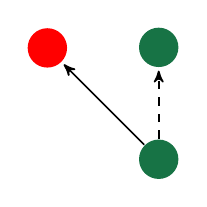
\begin{tikzpicture}[->,>=stealth',shorten >=1pt,auto,node distance=2cm,semithick]
  \tikzstyle{every state}=[draw=none]

  \node[state, fill=darkspringgreen,minimum size=.5cm] 	     (A)                    {};
  \node[state, fill=red,minimum size=.5cm]         (B) [above left of=A] {};
 % \node[state, fill=darkspringgreen,minimum size=.5cm]         (C) [below right of=A] {};
  \node[state, fill=darkspringgreen,minimum size=.5cm] 	     (D) [above =.9cm of A]                   {};

  \path[dashed] (A) edge              (D);
 %           	edge               (C);
  \path[->] (A) edge (B);

      \end{tikzpicture}
          \caption{Primary meristem transitioning to one vegetative meristem and generating one primary meristem.} 
  \end{subfigure}
              \hspace{\fill}
%% PRIMARY MERISTEM PRODUCING INFLORESCENCE MERISTEM
\begin{subfigure}{.25\textwidth}
    \centering
      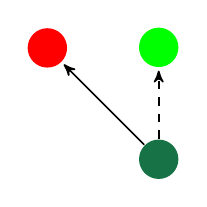
\begin{tikzpicture}[->,>=stealth',shorten >=1pt,auto,node distance=2cm,
                    semithick]

  \node[state, fill = darkspringgreen, draw = none,minimum size=.5cm] (A)                    {};
  \node[state, fill = red, draw = none,minimum size=.5cm]         (B) [above left of=A] {};
 % \node[state, fill = orange, draw = none,minimum size=.5cm]         (C) [above right of=A] {};
  \node[state, fill=green, draw = none,minimum size=.5cm] 	     (C) [above =.9cm of A]                   {};

  \path[dashed] (A) edge              (C);
  \path[->] (A) edge (B);

      \end{tikzpicture}
    \caption{Primary meristem transitioning to one vegetative meristem, and generating one inflorescence meristem.}
      \end{subfigure}
          \hspace{\fill}
%% PRIMARY MERISTEM PRODUCING INFLORESCENCE MERISTEM
      \begin{subfigure}{.25\textwidth}
% stem cell expansion
\centering
% stem cell expansion
      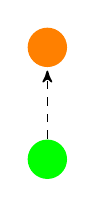
\begin{tikzpicture}[->,>=stealth',shorten >=1pt,auto,node distance=2cm,
                    semithick]

  \node[state, fill = green, draw = none,minimum size=.5cm] (A)                    {};
  \node[state, fill = orange, draw = none,minimum size=.5cm]         (B) [above =.9cm of A] {};
 % \node[state, fill = orange, draw = none,minimum size=.5cm]         (C) [below right of=A] {};

  \path[dashed] (A) edge              (B);
% \path (A) edge		     (B);

      \end{tikzpicture}
    \caption{Inflorescence meristem generating a floral meristem}
  \end{subfigure}
        \caption{Meristem transitions in an unbranched plant with a determinate inflorescence.}
    \label{fig:transitions-unbranched-determinate}
\end{figure}

The optimal control problem we are interested in is
%
\begin{align}
\max_{u} &  \int_0^T  \log( F(t) ) dt  \nonumber \\
\mathrm{subject\ to\ } 
& \dot{P} = - [q(t) V] [(1 - p(t)) P ] , \nonumber \\
& \dot{V} = [q(t) V] [ p(t) P]  + [q(t) V] [(1 - p(t)) P] , \nonumber \\ 
& \dot{I} = [q(t) V] [( 1-p(t) ) P], \nonumber \\ 
& \dot{F} = [(1-q(t)) V] I , \nonumber \\ 
& P(0) > 0;\ V(0),\ I(0),\ F(0) \geq 0, \nonumber \\
& 0 \leq p(t), q(t) \leq 1.  
\end{align}
%
\begin{table}[hbt!]
\footnotesize
\begin{tabularx}{\linewidth}{|l|X|}
\hline
\textbf{Term} & \textbf{Description} \\ \hline
 P    & Primary meristems            \\ \hline
 V   &  Vegetative biomass         \\ \hline
 I   &  Inflorescence meristems          \\ \hline
 F   &  Floral meristems          \\ \hline
 $p$  &  The probability that a primary meristem division produces a primary and vegetative meristem. A primary meristem division either produces a primary and vegetative meristem (Figure \ref{fig:transitions-unbranched-determinate}A) or an inflorescence and vegetative meristem (Figure \ref{fig:transitions-unbranched-determinate}B).      \\ \hline
 $q$   &  The fraction of photosynthate that is allocated to vegetative growth. Here, vegetative growth consists of primary meristem divisions. Any photosynthate not allocated to primary meristem divisions is allocated to inflorescence meristem divisions.         \\ \hline
\end{tabularx}
\end{table}
%

\noindent The Hamiltonian is 
%
\begin{align}
H = \log F +
((PV \lambda_1-PV \lambda_3)p-IV \lambda_4+PV \lambda_3+PV \lambda_2-PV \lambda_1)q+IV \lambda_4
\end{align}
%
The optimality conditions are
%
\begin{align}
& \frac{\partial H}{\partial p} = (PV)( \lambda_1 - \lambda_3)q = 0\ \mathrm{at}\ p^* \\
&\frac{\partial H}{\partial q} =  (PV)( \lambda_1- \lambda_3)p-IV \lambda_4+PV \lambda_3+PV \lambda_2-PV \lambda_1 = 0\ \mathrm{at}\ q^*
\end{align}
%
The transversality condition is
%
\begin{align}
\lambda_1(T) = \lambda_2(T) = \lambda_3(T) = \lambda_4(T) = 0.
\end{align}
%
The adjoint equations are
%
\begin{align}
&-\frac{\partial H}{\partial P} = \dot{\lambda_1}  = -((V \lambda_1-V \lambda_3)p+V \lambda_3+V \lambda_2-V \lambda_1)q \nonumber \\
&-\frac{\partial H}{\partial V} = \dot{\lambda_2}  = -((P \lambda_1-P \lambda_3)p-I \lambda_4+P \lambda_3+P \lambda_2-P \lambda_1)q-I \lambda_4  \nonumber\\
&-\frac{\partial H}{\partial I} = \dot{\lambda_3}  = V \lambda_4q-V \lambda_4 \nonumber \\
&-\frac{\partial H}{\partial L} = \dot{\lambda_4}  = -\frac{1}{F}  
\end{align}
%

I used an adapted forward-backward sweep. The figures on the following pages summarize some solutions for different initial conditions and show the general trajectory of state variables and adjoint variables.

 \begin{figure}[h]
   \centering
    \begin{subfigure}[t]{0.45\textwidth}
        \centering
       \includegraphics[width=\linewidth]{../../figures/unbranched-determinate-P=1-V=2,uniform(0,5)}  
        \caption{...} \label{fig:...}
    \end{subfigure}
    \hfill
    \begin{subfigure}[t]{0.45\textwidth}
        \centering
       \includegraphics[width=\linewidth]{../../figures/unbranched-determinate-P=1-V=1,uniform(0,5)}  
        \caption{...} \label{fig:...}
    \end{subfigure}
     \centering
    \begin{subfigure}[t]{0.45\textwidth}
        \centering
       \includegraphics[width=\linewidth]{../../figures/unbranched-determinate-P=1-V=05,uniform(0,5)}  
        \caption{...} \label{fig:...}
    \end{subfigure}
    \hfill
    \begin{subfigure}[t]{0.45\textwidth}
        \centering
       \includegraphics[width=\linewidth]{../../figures/unbranched-determinate-P=1-V=01,uniform(0,5)}  
        \caption{...} \label{fig:...}
    \end{subfigure}
        \caption{Trajectories of controls $p$ (solid line) and $q$ (dashed line) for a range of initial conditions. The optimal control suggests no division of primary meristems ($p(t)=0$) initially with oscillating allocation of photosynthate to vegetative growth. I cut off the solutions at 15000 iterations, so the controls in Panel d have not converged. See next two pages for figures corresponding to state trajectories and adjoint variables for Panel d.} \label{fig:...}
\end{figure}

 \begin{figure}[h]
        \centering
       \includegraphics[width=\linewidth]{../../figures/unbranched-determinate-states}  
        \caption{Trajectories of state variables for the case where the initial conditions are $P(0)=1,\ V(0)=0.1,\ I(0)=0,\ F(0)=0$.} \label{fig:...}
\end{figure}

 \begin{figure}[h]
        \centering
       \includegraphics[width=\linewidth]{../../figures/unbranched-determinate-adjoints}  
        \caption{Trajectories of adjoint variables for the case where the initial conditions are $P(0)=1,\ V(0)=0.1,\ I(0)=0,\ F(0)=0$.} \label{fig:...}
\end{figure}

\clearpage
\newpage

\section*{Unbranched, determinate case (budget constraint)}


\begin{figure}[hbt!]
%% PRIMARY MERISTEM PRODUCING PRIMARY MERISTEM
  \begin{subfigure}{.25\textwidth}
  \centering
    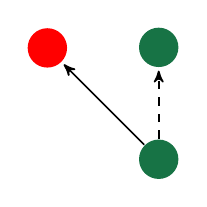
\begin{tikzpicture}[->,>=stealth',shorten >=1pt,auto,node distance=2cm,semithick]
  \tikzstyle{every state}=[draw=none]

  \node[state, fill=darkspringgreen,minimum size=.5cm] 	     (A)                    {};
  \node[state, fill=red,minimum size=.5cm]         (B) [above left of=A] {};
 % \node[state, fill=darkspringgreen,minimum size=.5cm]         (C) [below right of=A] {};
  \node[state, fill=darkspringgreen,minimum size=.5cm] 	     (D) [above =.9cm of A]                   {};

  \path[dashed] (A) edge              (D);
 %           	edge               (C);
  \path[->] (A) edge (B);

      \end{tikzpicture}
          \caption{Primary meristem transitioning to one vegetative meristem and generating one primary meristem.} 
  \end{subfigure}
              \hspace{\fill}
%% PRIMARY MERISTEM PRODUCING INFLORESCENCE MERISTEM
\begin{subfigure}{.25\textwidth}
    \centering
      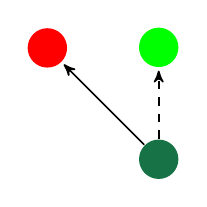
\begin{tikzpicture}[->,>=stealth',shorten >=1pt,auto,node distance=2cm,
                    semithick]

  \node[state, fill = darkspringgreen, draw = none,minimum size=.5cm] (A)                    {};
  \node[state, fill = red, draw = none,minimum size=.5cm]         (B) [above left of=A] {};
 % \node[state, fill = orange, draw = none,minimum size=.5cm]         (C) [above right of=A] {};
  \node[state, fill=green, draw = none,minimum size=.5cm] 	     (C) [above =.9cm of A]                   {};

  \path[dashed] (A) edge              (C);
  \path[->] (A) edge (B);

      \end{tikzpicture}
    \caption{Primary meristem transitioning to one vegetative meristem, and generating one inflorescence meristem.}
      \end{subfigure}
          \hspace{\fill}
%% PRIMARY MERISTEM PRODUCING INFLORESCENCE MERISTEM
      \begin{subfigure}{.25\textwidth}
% stem cell expansion
\centering
% stem cell expansion
      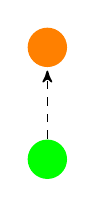
\begin{tikzpicture}[->,>=stealth',shorten >=1pt,auto,node distance=2cm,
                    semithick]

  \node[state, fill = green, draw = none,minimum size=.5cm] (A)                    {};
  \node[state, fill = orange, draw = none,minimum size=.5cm]         (B) [above =.9cm of A] {};
 % \node[state, fill = orange, draw = none,minimum size=.5cm]         (C) [below right of=A] {};

  \path[dashed] (A) edge              (B);
% \path (A) edge		     (B);

      \end{tikzpicture}
    \caption{Inflorescence meristem generating a floral meristem}
  \end{subfigure}
        \caption{Meristem transitions in an unbranched plant with a determinate inflorescence.}
    \label{fig:transitions-unbranched-determinate}
\end{figure}

%
\begin{table}[hbt!]
\footnotesize
\begin{tabularx}{\linewidth}{|l|X|}
\hline
\textbf{Term} & \textbf{Description} \\ \hline
 P    & Primary meristems            \\ \hline
 V   &  Vegetative biomass         \\ \hline
 I   &  Inflorescence meristems          \\ \hline
 F   &  Floral meristems          \\ \hline
 $\beta_1(t)$  &  The per-capita rate of division by primary meristems.     \\ \hline
  $\beta_2(t)$  &  The per-capita rate of division by inflorescence meristems.     \\ \hline
 $u(t)$   &  The probability that a primary meristem division produces a primary and vegetative meristem (Figure 1A).       \\ \hline
  $1-u(t)$   &  The probability that a primary meristem division produces an inflorescence and a vegetative meristem (Figure 1B).       \\ \hline
\end{tabularx}
\end{table}

The optimal control problem we are interested in is
%
\begin{align}
\max_{u} &  \int_0^T  \log( F(t) ) dt  \nonumber \\
\mathrm{subject\ to\ } 
& \dot{P} = - [\beta_1(t)] [(1 - u(t)) P ] , \nonumber \\
& \dot{V} = [\beta_1(t)] [ u(t) P]  + [\beta_1(t)] [(1 - u(t)) P] = \beta_1 [P] , \nonumber \\ 
& \dot{I} = [\beta_1(t)] [( 1-u(t) ) P] - [\beta_2(t)] I, \nonumber \\ 
& \dot{F} = [\beta_2(t)] I , \nonumber \\ 
& P(0) > 0;\ V(0),\ I(0),\ F(0) \geq 0, \nonumber \\
& 0 \le \beta_1(t), \beta_2(t) \le M & \mbox{ Meristem constraint}  \nonumber \\
& 0 \le \beta_1(t) P + \beta_2(t) I \le V & \mbox{ Resource constraint} \nonumber \\
& 0 \leq u(t) \leq 1.  
\end{align}



\noindent The Hamiltonian is 
%
\begin{align}
H = \log F + \lambda_1 [ - \beta_1 (1-u) P ] + \lambda_2 [ \beta_1 P ]  + \lambda_3 [ \beta_1 (1-u) P - \beta_2 I ] + \lambda_4 [ \beta_2 I ]
\end{align}
%
The optimality conditions are
%
\begin{align}
& \frac{\partial H}{\partial u} = (\lambda_1 - \lambda_3) \beta_1 P = 0\ \mathrm{at}\ \beta_1^*, \beta_2^* \\
&\frac{\partial H}{\partial \beta_1} =  (\lambda_3(1-u) - \lambda_1 (1-u) + \lambda_2) P = 0\ \mathrm{at}\ u^*, \beta_2^* \\
&\frac{\partial H}{\partial \beta_2} =  (\lambda_4 - \lambda_3) I = 0\ \mathrm{at}\ u^*, \beta_1^*
\end{align}
%
The transversality condition is
%
\begin{align}
\lambda_1(T) = \lambda_2(T) = \lambda_3(T) = \lambda_4(T) = 0.
\end{align}
%
The adjoint equations are
%
\begin{align}
&-\frac{\partial H}{\partial P} = \dot{\lambda_1}  = \beta_1 ( \lambda_1 (1-u) - \lambda_2 - \lambda_3 (1-u) ) \nonumber \\
&-\frac{\partial H}{\partial V} = \dot{\lambda_2}  = 0  \nonumber\\
&-\frac{\partial H}{\partial I} = \dot{\lambda_3}  = \beta_2(\lambda_3-\lambda_4) \nonumber \\
&-\frac{\partial H}{\partial L} = \dot{\lambda_4}  = -\frac{1}{F}  
\end{align}
%


%The constraints on $\beta_1, \beta_2$ are as shown below. The square is the meristem constraint, the diagonal line is the resource constraint: $(\beta_1, \beta_2)$ needs to be below the line (which has infinite length but I've only drawn part of it). The meristem constraint is constant over time. The resource constraint line moves because it depends on the values of $P(t),I(t)$ and $V(t)$. 

\smallskip 

%\centerline{\includegraphics[width=5in]{ConstraintDiagram.jpg}}

% I predict that when you work through the Hamiltonian etc., you will discover that increasing $\beta_1$ and/or $\beta_2$ is always beneficial (i.e., this increases the Hamiltonian). In checking to see if this is true, you can assume that the $\lambda$'s are always positive, because that is implied in this model by their interpretation as shadow prices. 

%If my prediction is right, then in Case 1 the optimal $\beta$s are always on the portion of the resource constraint line inside the meristem constraint box; and in Case 2 the optimal $\beta$s are $(M,M)$, the top right corner of the meristem constraint. 

% I think ?augmented Hamiltonian? is just a device for maximizing the ordinary Hamiltonian subject to the constraints, in the same way that Lagrange multipliers are a device for maximizing a function subject to constraints. In your case, it may be easier not to take the augmented Hamiltonian approach. If my hunch is right the maximum of the Hamiltonian as a function of (beta1,beta2) is always on the resource constraint curve or at the meristem constraint point (M,M). In the latter case there?s nothing more to do, in the former we can (at each time point) express beta2 as a function of beta1 on the resource constraint curve, and find the gradient of the Hamiltonian with respect to beta1 along the curve.

\clearpage
\newpage

\section*{Unbranched, determinate case without resource constraint}

To start, if we ignore the resource constraint the problem becomes one of solving 
%
\begin{align}
\max_{u} &  \int_0^T  \log( F(t) ) dt  \nonumber \\
\mathrm{subject\ to\ } 
& \dot{P} = - [\beta_1(t)] [(1 - u(t)) P ] , \nonumber \\
& \dot{V} = [\beta_1(t)] [ u(t) P]  + [\beta_1(t)] [(1 - u(t)) P] = \beta_1 [P] , \nonumber \\ 
& \dot{I} = [\beta_1(t)] [( 1-u(t) ) P] - [\beta_2(t)] I, \nonumber \\ 
& \dot{F} = [\beta_2(t)] I , \nonumber \\ 
& P(0) > 0;\ V(0),\ I(0),\ F(0) \geq 0, & \mbox{System of ODEs, initial conditions}  \nonumber \\
& 0 \le \beta_1(t), \beta_2(t) \le M & \mbox{ Meristem constraint}  \nonumber \\
% & 0 \le \beta_1(t) P + \beta_2(t) I \le V & \mbox{ Resource constraint} \nonumber \\
& 0 \leq u(t) \leq 1 & \mbox{Control constraint} \nonumber.  
\end{align}

We can write the Hamiltonian as
%
\begin{align}
& H = \log F + \lambda_1 [ - \beta_1 (1-u) P ] + \lambda_2 [ \beta_1 P ]  + \lambda_3 [ \beta_1 (1-u) P - \beta_2 I ] + \lambda_4 [ \beta_2 I ] 
\end{align}
%
The derivative of the Hamiltonian with respect to the control gives us our switching functions
%
\begin{align}
& \frac{\partial H}{\partial u} = (\lambda_1 - \lambda_3) \beta_1 P = \Phi_1(t) \ \mathrm{at}\ \beta_1^*, \beta_2^* \\
&\frac{\partial H}{\partial \beta_1} =  (\lambda_3(1-u) - \lambda_1 (1-u) + \lambda_2 ) P = \Phi_2(t) \ \mathrm{at}\ u^*, \beta_2^* \\
&\frac{\partial H}{\partial \beta_2} =  (\lambda_4 - \lambda_3) I = \Phi_3(t) \ \mathrm{at}\ u^*, \beta_1^*
\end{align}
%
The adjoint equations are
%
\begin{align}
&-\frac{\partial H}{\partial P} = \dot{\lambda_1}  = \beta_1 ( \lambda_1 (1-u) - \lambda_2 - \lambda_3 (1-u) ) \nonumber \\
&-\frac{\partial H}{\partial V} = \dot{\lambda_2}  = 0  \nonumber\\
&-\frac{\partial H}{\partial I} = \dot{\lambda_3}  = \beta_2(\lambda_3-\lambda_4) \nonumber \\
&-\frac{\partial H}{\partial F} = \dot{\lambda_4}  = -\frac{1}{F}  
\end{align}
The transversality condition is
%
\begin{align}
\lambda_1(T) = \lambda_2(T) = \lambda_3(T) = \lambda_4(T) = 0.
\end{align}
%
Without a resource constraint, the optimal strategy is $u=0$ and $\beta_1=\beta_2=M$ at all times. In this model, meristems have no value as branches (there is no branching) or as bearers of vegetative, photosynthetic biomass. We get here by first considering $\beta_2$, which we find to be bang-bang. We then consider $u$ and $\beta_1$ jointly. I have not been able to analyze this completely but the partial derivatives with respect to the Hamiltonian both suggest that decreases in $u$ and increases $\beta_1$ increase $H$ at all times, suggesting that both are bang-bang as well.

\clearpage
\newpage

\section*{Unbranched, determinate case with resource constraint}

Including a resource constraint makes this a problem of the kind discussed by Kamien and Schwartz in State Variable Inequality Constraints (p 231) and by Chiang in Optimal Control with Constraints (p 300). Kamien and Schwartz solve these problems with the following approach.
%
\begin{align}
\max &  \int_{t_0}^{t_1}  f(t,x,u) dt + \phi(x(t_1)) \nonumber \\
\mathrm{subject\ to\ } 
& \dot{x} = g(t,x,u), \ x(t_0) = x_0 \nonumber & \mbox{System of ODEs, initial conditions}  \nonumber \\
& k(t,x) \geq 0 & \mbox{ State variable inequality constraint}  \nonumber
\end{align}

To solve the problem, associate a multiplier $\lambda$ with the system of ODEs and a multiplier $\eta$ with the state variable constraint. The Hamiltonian is then
%
\begin{align}
H = f(t,x,u) + \lambda g(t,x,u) + \eta k(t,x) \nonumber
\end{align}

Necessary conditions for optimality include satisfying the system of ODEs, the state variable constraint, and
%
\begin{align}
& \frac{\partial H}{\partial u}  = \frac{\partial f}{\partial u} + \lambda \frac{\partial g}{\partial u} = 0  & \mbox{Optimality conditions} \nonumber \\
 & \frac{\partial H}{\partial x}  = - \dot{\lambda} = \frac{\partial f}{\partial x} + \lambda \frac{\partial g}{\partial x} + \eta \frac{\partial k}{\partial x} & \mbox{Adjoint equations} \nonumber \\
& \lambda(t_1)  = \frac{\partial \phi}{\partial x}  (x(t_1))  & \mbox{Transversality condition/payoff} \nonumber \\
& \eta \geq 0, \eta k(t,x) = 0  & \mbox{complementary slackness conditions} \nonumber \\
\end{align}

Chiang takes the following approach:

We now rewrite our maximization problem, this time including a resource constraint
%
\begin{align}
\max_{u} &  \int_0^T  \log( F(t) ) dt  \nonumber \\
\mathrm{subject\ to\ } 
& \dot{P} = - [\beta_1(t)] [(1 - u(t)) P ] , \nonumber \\
& \dot{V} = [\beta_1(t)] [ u(t) P]  + [\beta_1(t)] [(1 - u(t)) P] = \beta_1 [P] , \nonumber \\ 
& \dot{I} = [\beta_1(t)] [( 1-u(t) ) P] - [\beta_2(t)] I, \nonumber \\ 
& \dot{F} = [\beta_2(t)] I , \nonumber \\ 
& P(0) > 0;\ V(0),\ I(0),\ F(0) \geq 0, & \mbox{System of ODEs, initial conditions}  \nonumber \\
& 0 \le \beta_1(t), \beta_2(t) \le M & \mbox{ Meristem constraint}  \nonumber \\
& 0 \le \beta_1(t) P + \beta_2(t) I \le V & \mbox{ Resource constraint} \nonumber \\
& 0 \leq u(t) \leq 1 & \mbox{Control constraint} \nonumber.  
\end{align}

The Hamiltonian is then 
%
\begin{align}
& H = \log F + \lambda_1 [ - \beta_1 (1-u) P ] + \lambda_2 [ \beta_1 P ]  + \lambda_3 [ \beta_1 (1-u) P - \beta_2 I ] + \lambda_4 [ \beta_2 I ] + \eta [V - (\beta_1 P + \beta_2 I) ]
\end{align}
%
The optimality conditions are
%
\begin{align}
& \frac{\partial H}{\partial u} = (\lambda_1 - \lambda_3) \beta_1 P = 0\ \mathrm{at}\ \beta_1^*, \beta_2^* \\
&\frac{\partial H}{\partial \beta_1} =  (\lambda_3(1-u) - \lambda_1 (1-u) + \lambda_2 - \eta) P = 0\ \mathrm{at}\ u^*, \beta_2^* \\
&\frac{\partial H}{\partial \beta_2} =  (\lambda_4 - \lambda_3 - \eta) I = 0\ \mathrm{at}\ u^*, \beta_1^*
\end{align}
%
The transversality condition is
%
\begin{align}
\lambda_1(T) = \lambda_2(T) = \lambda_3(T) = \lambda_4(T) = 0.
\end{align}
%
The adjoint equations are
%
\begin{align}
&-\frac{\partial H}{\partial P} = \dot{\lambda_1}  = \beta_1 ( \lambda_1 (1-u) - \lambda_2 - \lambda_3 (1-u) + \eta \beta_1 ) \nonumber \\
&-\frac{\partial H}{\partial V} = \dot{\lambda_2}  = - \eta  \nonumber\\
&-\frac{\partial H}{\partial I} = \dot{\lambda_3}  = \beta_2(\eta + \lambda_3-\lambda_4) \nonumber \\
&-\frac{\partial H}{\partial F} = \dot{\lambda_4}  = -\frac{1}{F}  
\end{align}
%
And 
\begin{align}
& \eta \geq 0,\ \eta [V-(\beta_1 P + \beta_2 I) ] = 0  
\end{align}
% 
From the above equation,  $\eta = 0$ when $V - (\beta_1 P + \beta_2 I) > 0 $ (off the constraint). On the other hand, $\eta > 0$ when $V - (\beta_1 P + \beta_2 I) \leq 0$ (on the constraint).


When we are not on the boundary ($V-(\beta_1 P + \beta_2 I)>0$)
We do the following on the boundary
%
\begin{align}
\phi = \frac{ (P(\lambda_3 - \lambda_1) (1-u) + \lambda_2 ) - (I(\lambda_4 - \lambda_3) }{P - I}
\end{align}
%



\iffalse
\clearpage
\newpage


\section*{Branched, determinate case}

\begin{figure}[hbt!]
%% PRIMARY MERISTEM PRODUCING PRIMARY MERISTEM
  \begin{subfigure}{.25\textwidth}
  \centering
    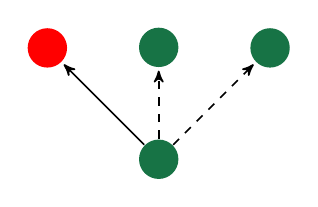
\begin{tikzpicture}[->,>=stealth',shorten >=1pt,auto,node distance=2cm,semithick]
  \tikzstyle{every state}=[draw=none]

  \node[state, fill=darkspringgreen,minimum size=.5cm] 	     (A)                    {};
  \node[state, fill=red,minimum size=.5cm]         (B) [above left of=A] {};
  \node[state, fill=darkspringgreen,minimum size=.5cm]         (C) [above right of=A] {};
  \node[state, fill=darkspringgreen,minimum size=.5cm] 	     (D) [above =.9cm of A]                   {};

  \path[dashed] (A) edge              (D)
            	edge               (C);
  \path[->] (A) edge (B);

      \end{tikzpicture}
          \caption{Primary meristem transitioning to one vegetative meristem and generating two primary meristems.} 
  \end{subfigure}
              \hspace{\fill}
%% PRIMARY MERISTEM PRODUCING INFLORESCENCE MERISTEM
\begin{subfigure}{.25\textwidth}
    \centering
      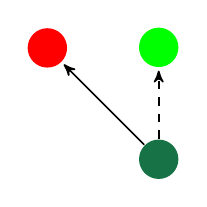
\begin{tikzpicture}[->,>=stealth',shorten >=1pt,auto,node distance=2cm,
                    semithick]

  \node[state, fill = darkspringgreen, draw = none,minimum size=.5cm] (A)                    {};
  \node[state, fill = red, draw = none,minimum size=.5cm]         (B) [above left of=A] {};
 % \node[state, fill = orange, draw = none,minimum size=.5cm]         (C) [above right of=A] {};
  \node[state, fill=green, draw = none,minimum size=.5cm] 	     (C) [above =.9cm of A]                   {};

  \path[dashed] (A) edge              (C);
  \path[->] (A) edge (B);

      \end{tikzpicture}
    \caption{Primary meristem transitioning to one vegetative meristem, and generating one inflorescence meristem.}
      \end{subfigure}
          \hspace{\fill}
%% PRIMARY MERISTEM PRODUCING INFLORESCENCE MERISTEM
      \begin{subfigure}{.25\textwidth}
% stem cell expansion
\centering
% stem cell expansion
      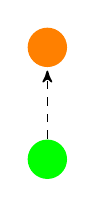
\begin{tikzpicture}[->,>=stealth',shorten >=1pt,auto,node distance=2cm,
                    semithick]

  \node[state, fill = green, draw = none,minimum size=.5cm] (A)                    {};
  \node[state, fill = orange, draw = none,minimum size=.5cm]         (B) [above =.9cm of A] {};
 % \node[state, fill = orange, draw = none,minimum size=.5cm]         (C) [below right of=A] {};

  \path[dashed] (A) edge              (B);
% \path (A) edge		     (B);

      \end{tikzpicture}
    \caption{Inflorescence meristem generating a floral meristem}
  \end{subfigure}
        \caption{Meristem transitions in an unbranched plant with a determinate inflorescence.}
    \label{fig:transitions-determinate}
\end{figure}


The optimal control problem we are interested in is
%
\begin{align}
\max_{u} &  \int_0^T  \log( F(t) ) dt  \nonumber \\
\mathrm{subject\ to\ } 
& \dot{P} = [q(t) V] [p(t) P] - [q(t) V] [(1 - p(t)) P ] , \nonumber \\
& \dot{V} = [q(t) V] [ p(t) P]  + [q(t) V] [(1 - p(t)) P] , \nonumber \\ 
& \dot{I} = [q(t) V] [( 1-p(t) ) P], \nonumber \\ 
& \dot{F} = [(1-q(t)) V] I , \nonumber \\ 
& P(0) > 0;\ V(0),\ I(0),\ F(0) \geq 0, \nonumber \\
& 0 \leq p(t), q(t) \leq 1.  
\end{align}
%
\begin{table}[hbt!]
\footnotesize
\begin{tabularx}{\linewidth}{|l|X|}
\hline
\textbf{Term} & \textbf{Description} \\ \hline
 P    & Primary meristems            \\ \hline
 V   &  Vegetative biomass         \\ \hline
 I   &  Inflorescence meristems          \\ \hline
 F   &  Floral meristems          \\ \hline
 $p$  &  The probability that a primary meristem division produces a primary and vegetative meristem. A primary meristem division either produces a primary and vegetative meristem (Figure \ref{fig:transitions-unbranched-determinate}A) or an inflorescence and vegetative meristem (Figure \ref{fig:transitions-unbranched-determinate}B).      \\ \hline
 $q$   &  The fraction of photosynthate that is allocated to vegetative growth. Here, vegetative growth consists of primary meristem divisions. Any photosynthate not allocated to primary meristem divisions is allocated to inflorescence meristem divisions.         \\ \hline
\end{tabularx}
\end{table}
%
\noindent The Hamiltonian is 
%
\begin{align}
H = \log F +
((2PV \lambda_1-PV \lambda_3 )p-IV \lambda_4+PV \lambda_3+PV \lambda_2-PV \lambda_1)q+IV \lambda_4
\end{align}
%
The optimality conditions are
%
\begin{align}
& \frac{\partial H}{\partial p} = (PV)( 2\lambda_1 - \lambda_3)q = 0\ \mathrm{at}\ p^* \\
&\frac{\partial H}{\partial q} =  (PV) ( 2\lambda_1- \lambda_3)p-IV \lambda_4+PV \lambda_3+PV \lambda_2-PV \lambda_1 = 0\ \mathrm{at}\ q^* 
\end{align}
%
The transversality condition is
%
\begin{align}
\lambda_1(T) = \lambda_2(T) = \lambda_3(T) = \lambda_4(T) = 0.
\end{align}
%
The adjoint equations are
%
\begin{align}
&-\frac{\partial H}{\partial P} = \dot{\lambda_1}  = -((2 V \lambda_1-V \lambda_3)p+V \lambda_3+V \lambda_2-V \lambda_1)q \nonumber \\
&-\frac{\partial H}{\partial V} = \dot{\lambda_2}  = -((2 P \lambda_1-P \lambda_3)p-I \lambda_4+P \lambda_3+P \lambda_2-P \lambda_1)q-I \lambda_4  \nonumber\\
&-\frac{\partial H}{\partial I} = \dot{\lambda_3}  = V \lambda_4q-V \lambda_4 \nonumber \\
&-\frac{\partial H}{\partial L} = \dot{\lambda_4}  = -\frac{1}{F}  
\end{align}

\clearpage
\newpage


\section*{Unbranched, indeterminate case}

\begin{figure}[hbt!]
%% PRIMARY MERISTEM PRODUCING PRIMARY MERISTEM
  \begin{subfigure}{.25\textwidth}
  \centering
    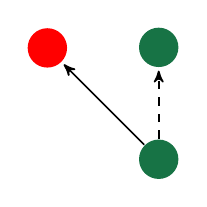
\begin{tikzpicture}[->,>=stealth',shorten >=1pt,auto,node distance=2cm,semithick]
  \tikzstyle{every state}=[draw=none]

  \node[state, fill=darkspringgreen,minimum size=.5cm] 	     (A)                    {};
  \node[state, fill=red,minimum size=.5cm]         (B) [above left of=A] {};
 % \node[state, fill=darkspringgreen,minimum size=.5cm]         (C) [below right of=A] {};
  \node[state, fill=darkspringgreen,minimum size=.5cm] 	     (D) [above =.9cm of A]                   {};

  \path[dashed] (A) edge              (D);
 %           	edge               (C);
  \path[->] (A) edge (B);

      \end{tikzpicture}
          \caption{Primary meristem transitioning to one vegetative meristem and generating one primary meristem.} 
  \end{subfigure}
              \hspace{\fill}
%% PRIMARY MERISTEM PRODUCING INFLORESCENCE MERISTEM
\begin{subfigure}{.25\textwidth}
    \centering
      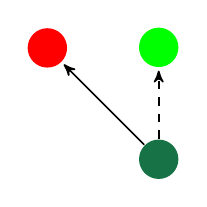
\begin{tikzpicture}[->,>=stealth',shorten >=1pt,auto,node distance=2cm,
                    semithick]

  \node[state, fill = darkspringgreen, draw = none,minimum size=.5cm] (A)                    {};
  \node[state, fill = red, draw = none,minimum size=.5cm]         (B) [above left of=A] {};
 % \node[state, fill = orange, draw = none,minimum size=.5cm]         (C) [above right of=A] {};
  \node[state, fill=green, draw = none,minimum size=.5cm] 	     (C) [above =.9cm of A]                   {};

  \path[dashed] (A) edge              (C);
  \path[->] (A) edge (B);

      \end{tikzpicture}
    \caption{Primary meristem transitioning to one vegetative meristem, and generating one inflorescence meristem.}
      \end{subfigure}
          \hspace{\fill}
%% INFLORESCENCE MERISTEM PRODUCING FLORAL MERISTEM
      \begin{subfigure}{.25\textwidth}
% stem cell expansion
\centering
% stem cell expansion
      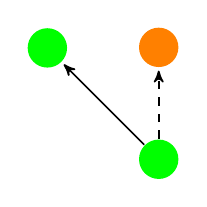
\begin{tikzpicture}[->,>=stealth',shorten >=1pt,auto,node distance=2cm,
                    semithick]

  \node[state, fill = green, draw = none,minimum size=.5cm] (A)                    {};
  \node[state, fill = orange, draw = none,minimum size=.5cm]         (B) [above =.9cm of A] {};
  \node[state, fill = green, draw = none,minimum size=.5cm]         (C) [above left of=A] {};

  \path[dashed] (A) edge              (B);
 \path (A) edge		     (C);

      \end{tikzpicture}
    \caption{Inflorescence meristem transitioning to one inflorescence meristem, and generating a floral meristem}
  \end{subfigure}
        \caption{Meristem transitions in an unbranched plant with an indeterminate inflorescence.}
    \label{fig:transitions-determinate}
\end{figure}




\clearpage
\newpage

\section*{Branched, indeterminate case}

\begin{figure}[hbt!]
%% PRIMARY MERISTEM PRODUCING PRIMARY MERISTEM
  \begin{subfigure}{.25\textwidth}
  \centering
    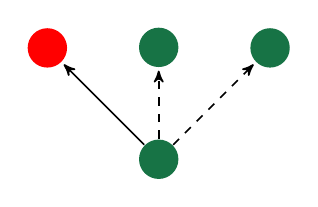
\begin{tikzpicture}[->,>=stealth',shorten >=1pt,auto,node distance=2cm,semithick]
  \tikzstyle{every state}=[draw=none]

  \node[state, fill=darkspringgreen,minimum size=.5cm] 	     (A)                    {};
  \node[state, fill=red,minimum size=.5cm]         (B) [above left of=A] {};
  \node[state, fill=darkspringgreen,minimum size=.5cm]         (C) [above right of=A] {};
  \node[state, fill=darkspringgreen,minimum size=.5cm] 	     (D) [above =.9cm of A]                   {};

  \path[dashed] (A) edge              (C)
            	(A) edge               (D);
  \path[->] (A) edge (B);

      \end{tikzpicture}
          \caption{Primary meristem transitioning to one vegetative meristem and generating two primary meristems.} 
  \end{subfigure}
              \hspace{\fill}
%% PRIMARY MERISTEM PRODUCING INFLORESCENCE MERISTEM
\begin{subfigure}{.25\textwidth}
    \centering
      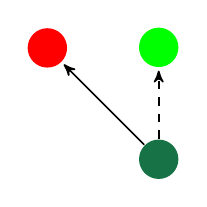
\begin{tikzpicture}[->,>=stealth',shorten >=1pt,auto,node distance=2cm,
                    semithick]

  \node[state, fill = darkspringgreen, draw = none,minimum size=.5cm] (A)                    {};
  \node[state, fill = red, draw = none,minimum size=.5cm]         (B) [above left of=A] {};
 % \node[state, fill = orange, draw = none,minimum size=.5cm]         (C) [above right of=A] {};
  \node[state, fill=green, draw = none,minimum size=.5cm] 	     (C) [above =.9cm of A]                   {};

  \path[dashed] (A) edge              (C);
  \path[->] (A) edge (B);

      \end{tikzpicture}
    \caption{Primary meristem transitioning to one vegetative meristem, and generating one inflorescence meristem.}
      \end{subfigure}
          \hspace{\fill}
%% INFLORESCENCE MERISTEM PRODUCING FLORAL MERISTEM
      \begin{subfigure}{.25\textwidth}
% stem cell expansion
\centering
% stem cell expansion
      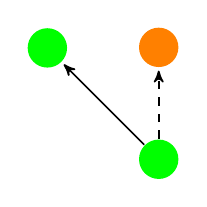
\begin{tikzpicture}[->,>=stealth',shorten >=1pt,auto,node distance=2cm,
                    semithick]

  \node[state, fill = green, draw = none,minimum size=.5cm] (A)                    {};
  \node[state, fill = orange, draw = none,minimum size=.5cm]         (B) [above =.9cm of A] {};
  \node[state, fill = green, draw = none,minimum size=.5cm]         (C) [above left of=A] {};

  \path[dashed] (A) edge              (B);
 \path (A) edge		     (C);

      \end{tikzpicture}
    \caption{Inflorescence meristem transitioning to one inflorescence meristem, and generating a floral meristem}
  \end{subfigure}
        \caption{Meristem transitions in an unbranched plant with an indeterminate inflorescence.}
    \label{fig:transitions-determinate}
\end{figure}

\fi


\end{document}